\begin{frame}
	\frametitle{Algoritmos de ordenação - baseados em seleção}
	\par A ideia é selecionar um elemento e já colocá-lo em sua posição correta definitiva evitando assim futuras permutações com o mesmo.
\end{frame}

\begin{frame}
	\frametitle{Algoritmos de ordenação - baseados em seleção}
	\begin{itemize}
		\item \textbf{Selection-Sort}
		\item \textbf{Heap-Sort}
	\end{itemize}
\end{frame}

\begin{frame}
	\frametitle{Algoritmos de ordenação - baseados em seleção}
	\framesubtitle{Selection-sort}
	\par É um algoritmo que seleciona o menor elemento do vetor e o coloca no início do mesmo, em seguida, seleciona o menor elemento do \textbf{vetor n-1} e o coloca no início desse vetor resultante. Esse algoritmo se repete até que o vetor esteja totalmente ordenado. 
	
	\par $55,33,12,01,19,10,70,25$	
	\par $\underbrace{55,33,12,\apontar{menor}{01},19,10,70,25}$
	\pause
	\par $\underbrace{\apontar{menor}{01},55,33,12,55,19,10,70,25}$
	\pause
	\par $01,\underbrace{55,33,12,55,19,\apontar{menor}{10},70,25}$
	\pause
	\par $01,\underbrace{\apontar{menor}{10},33,12,55,19,55,70,25}$
\end{frame}

\begin{frame}
	\frametitle{Algoritmos de ordenação - baseados em seleção}
	\framesubtitle{Selection-sort}
		\begin{columns}
		\begin{column}{0.5\textwidth}
			\par $01,\underbrace{\apontar{menor}{10},33,12,55,19,55,70,25}$
			\pause
			\par $01, 10, \underbrace{33,\apontar{menor}{12},55,19,55,70,25}$
			\pause
			\par $01, 10, \underbrace{\apontar{menor}{12},33,55,19,55,70,25}$
			\pause
			\par $01, 10, 12,\underbrace{33,55,\apontar{menor}{19},55,70,25}$
			\pause
			\par $01, 10, 12,\underbrace{\apontar{menor}{19},55,33,55,70,25}$
		\end{column}
		\begin{column}{0.5\textwidth}
			\par $01, 10, 12, 19,\underbrace{55,33,55,70,\apontar{menor}{25}}$
			\pause
			\par $01, 10, 12, 19,\underbrace{\apontar{menor}{25},33,55,70,55}$
			\pause
			\par $01, 10, 12, 19, 25, \underbrace{\apontar{menor}{33},55,70,55}$
			\pause
			\par $01, 10, 12, 19, 25, 33,\underbrace{\apontar{menor}{55},70,55}$
			\pause
			\par $01, 10, 12, 19, 25, 33, 55, \underbrace{70, \apontar{menor}{55}}$
			\pause
			\par $01, 10, 12, 19, 25, 33, 55, 55, 70 \leftarrow$ ordenado!
		\end{column}
	\end{columns}
\end{frame}

\begin{frame}
	\frametitle{Algoritmos de ordenação - baseados em seleção}
	\framesubtitle{Selection-sort - Exercício 0}
	\par Algoritmo:
	\lstinputlisting[language=C++]{../codigo/selectionSort.cpp}

	\par Determine o tempo de execução do \textit{Selection-sort} com seus respectivos melhores e piores tempos se houverem. Use a notação que melhor se encaixa à situação.
	\pause
	\par \textbf{Resposta:}
	\par $\Theta(n^2)$

\end{frame}

\begin{frame}
	\frametitle{Algoritmos de ordenação - baseados em seleção}
	\framesubtitle{Heap-sort}
	\par São algoritmos baseados em uma estrutura dados chamada de \textbf{Heap} que nada mais é do que um tipo de \textbf{árvore binária} de dados. É uma evolução do \textit{selection-sort}, no nosso caso vai trazer sempre em seu elemento raíz o maior valor do vetor (\textit{heap máximo}) e será balanceado a esquerda.
	\par Pode ser implementado de várias formas mas, como o objetivo aqui é ordenar um vetor, tal implementação não passará disso, portanto a árvore binária que representa esta estrutura de dados terá como nós filhos as expressões \ref{eq:fe} e \ref{eq:fd} e como nó pai \ref{eq:np}.
	\begin{equation}
		\label{eq:fe}
		filhoEsquerdo(k)=2k+1
	\end{equation}
	\begin{equation}
		\label{eq:fd}
		filhoDireito(k)=2k+2
	\end{equation}
	\begin{equation}
		\label{eq:np}
		pai(k)=\dfrac{k-1}{2}
	\end{equation}
\end{frame}
	
\begin{frame}
	\frametitle{Algoritmos de ordenação - baseados em seleção}
	\framesubtitle{Heap-sort}
	\par Decerto o ajuste do \textit{Heap} tem seu custo, no entanto, devido ao balanceamento da árvore tal custo é de ordem (descubra isso no exercício).
	\par Por fim, eis a definição do \textit{heap-sort}:
	\begin{itemize}
		\item construir o \textit{heap} máximo
		\item trocar a raiz (o maior elemento cuja localização é 0) com o elemento da última posição do vetor.
		\item diminuir o tamanho do \textit{heap} em 1
		\item rearranjar o \textit{heap} máximo se necessário
		\item repetir o processo n-1 vezes
	\end{itemize}
\end{frame}

\begin{frame}
	\frametitle{Algoritmos de ordenação - baseados em seleção}
	\framesubtitle{Heap-sort}
	\tikzset{
		heap/.style={
			every node/.style={circle,draw},
			level 1/.style={sibling distance=30mm},
			level 2/.style={sibling distance=15mm},
			level 3/.style={sibling distance=10mm},
			level 4/.style={sibling distance=5mm}
		},
		fontbf/.style={font=\bfseries}
	}
	\only<1>{
	\begin{columns}
		\begin{column}{0.5\textwidth}
			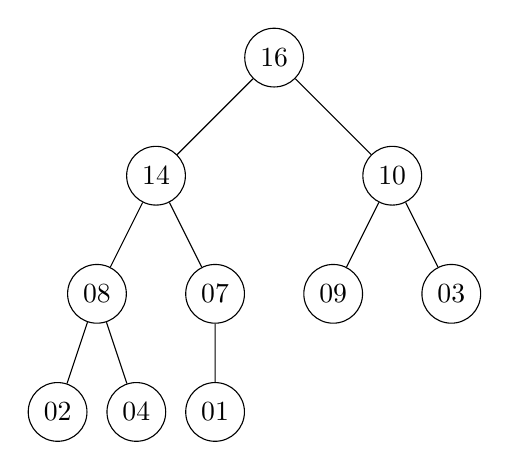
\begin{tikzpicture}[heap]
				\node {16}
				child{
					node{14}
					child{
						node{08}
						child{
							node{02}
						}
						child{
							node{04}
						}
					}
					child{
						node{07}
						child{
							node{01}
						}
					}
				}
				child{
					node{10}
					child{
						node{09}
					}
					child{
						node{03}
					}
				};
			\end{tikzpicture}
		\end{column}
		\begin{column}{0.5\textwidth}
			\par $
			\apontar{0}{16}, 
			\apontar{1}{14}, 
			\apontar{2}{10},  
			\apontar{3}{08}, 
			\apontar{4}{07}, 
			\apontar{5}{09},
			\apontar{6}{03}, 
			\apontar{7}{02},
			\apontar{8}{04}, 
			\apontar{9}{01}
			$
		\end{column}
	\end{columns}
}
	\only<2>{
	\begin{columns}
		\begin{column}{0.5\textwidth}
			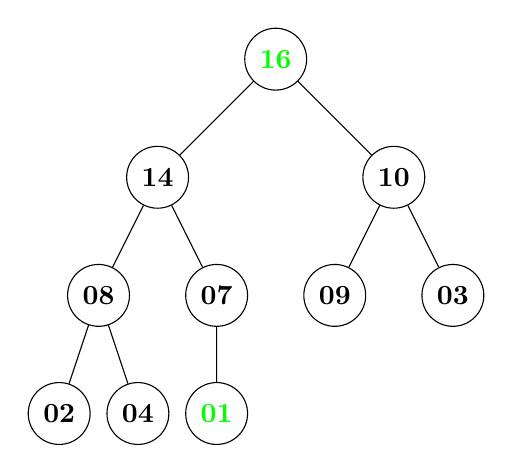
\begin{tikzpicture}[heap, fontbf]
				\node{\textcolor{green}{16}}
				child{
					node{14}
					child{
						node{08}
						child{
							node{02}
						}
						child{
							node{04}
						}
					}
					child{
						node{07}
						child{
							node{\textcolor{green}{01}}
						}
					}
				}
				child{
					node{10}
					child{
						node{09}
					}
					child{
						node{03}
					}
				};
			\end{tikzpicture}
		\end{column}
		\begin{column}{0.5\textwidth}
			\par $
			\apontar{0}{\textcolor{green}{16}}, 
			\apontar{1}{14}, 
			\apontar{2}{10},  
			\apontar{3}{08}, 
			\apontar{4}{07}, 
			\apontar{5}{09},
			\apontar{6}{03}, 
			\apontar{7}{02},
			\apontar{8}{04}, 
			\apontar{9}{\textcolor{green}{01}}
			$
		\end{column}
	\end{columns}
}
\only<3>{
	\begin{columns}
		\begin{column}{0.5\textwidth}
			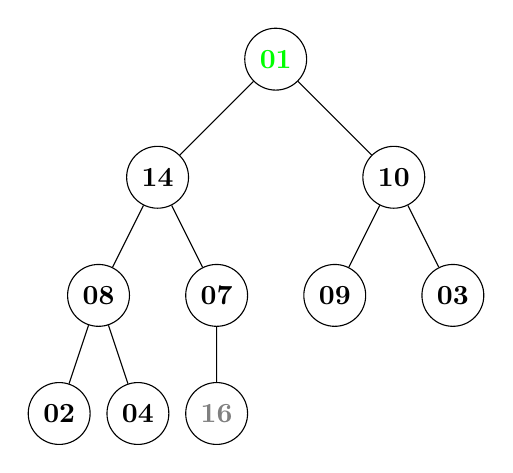
\begin{tikzpicture}[heap, fontbf]
				\node{\textcolor{green}{01}}
				child{
					node{14}
					child{
						node{08}
						child{
							node{02}
						}
						child{
							node{04}
						}
					}
					child{
						node{07}
						child{
							node{\textcolor{gray}{16}}
						}
					}
				}
				child{
					node{10}
					child{
						node{09}
					}
					child{
						node{03}
					}
				};
			\end{tikzpicture}
		\end{column}
		\begin{column}{0.5\textwidth}
			\par $
			\apontar{0}{\textcolor{green}{01}}, 
			\apontar{1}{14}, 
			\apontar{2}{10},  
			\apontar{3}{08}, 
			\apontar{4}{07}, 
			\apontar{5}{09},
			\apontar{6}{03}, 
			\apontar{7}{02},
			\apontar{8}{04}, 
			\apontar{9}{\textcolor{gray}{16}}
			$
		\end{column}
	\end{columns}
}
\only<4>{
	\par Ajustando o \textit{heap}
	\begin{columns}
		\begin{column}{0.5\textwidth}
			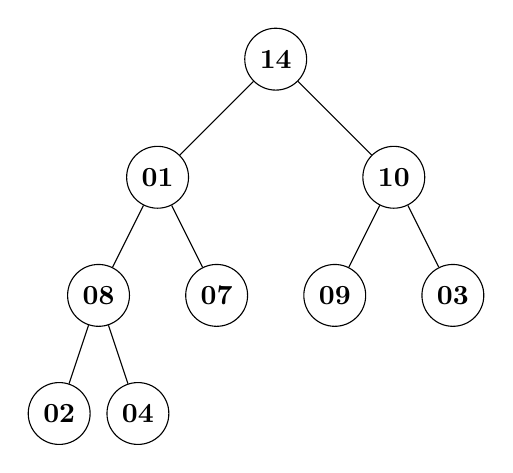
\begin{tikzpicture}[heap, fontbf]
				\node{14}
				child{
					node{01}
					child{
						node{08}
						child{
							node{02}
						}
						child{
							node{04}
						}
					}
					child{
						node{07}
					}
				}
				child{
					node{10}
					child{
						node{09}
					}
					child{
						node{03}
					}
				};
			\end{tikzpicture}
		\end{column}
		\begin{column}{0.5\textwidth}
			\par $
			\apontar{0}{14}, 
			\apontar{1}{01}, 
			\apontar{2}{10},  
			\apontar{3}{08}, 
			\apontar{4}{07}, 
			\apontar{5}{09},
			\apontar{6}{03}, 
			\apontar{7}{02},
			\apontar{8}{04}, 
			\apontar{9}{\textcolor{gray}{16}}
			$
		\end{column}
	\end{columns}
}
\only<5>{
	\par Ajustando o \textit{heap}
	\begin{columns}
		\begin{column}{0.5\textwidth}
			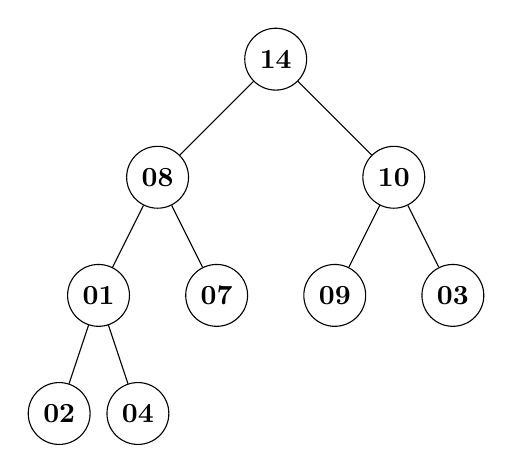
\begin{tikzpicture}[heap, fontbf]
				\node{14}
				child{
					node{08}
					child{
						node{01}
						child{
							node{02}
						}
						child{
							node{04}
						}
					}
					child{
						node{07}
					}
				}
				child{
					node{10}
					child{
						node{09}
					}
					child{
						node{03}
					}
				};
			\end{tikzpicture}
		\end{column}
		\begin{column}{0.5\textwidth}
			\par $
			\apontar{0}{14}, 
			\apontar{1}{08}, 
			\apontar{2}{10},  
			\apontar{3}{01}, 
			\apontar{4}{07}, 
			\apontar{5}{09},
			\apontar{6}{03}, 
			\apontar{7}{02},
			\apontar{8}{04}, 
			\apontar{9}{\textcolor{gray}{16}}
			$
		\end{column}
	\end{columns}
}
\only<6>{
	\par \textit{heap} ajustado!
	\begin{columns}
		\begin{column}{0.5\textwidth}
			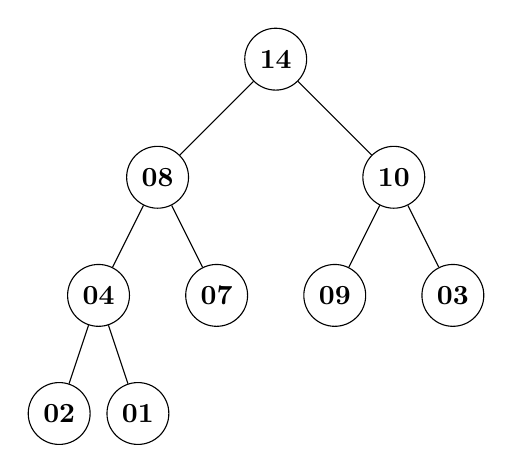
\begin{tikzpicture}[heap, fontbf]
				\node{14}
				child{
					node{08}
					child{
						node{04}
						child{
							node{02}
						}
						child{
							node{01}
						}
					}
					child{
						node{07}
					}
				}
				child{
					node{10}
					child{
						node{09}
					}
					child{
						node{03}
					}
				};
			\end{tikzpicture}
		\end{column}
		\begin{column}{0.5\textwidth}
			\par $
			\apontar{0}{14}, 
			\apontar{1}{08}, 
			\apontar{2}{10},  
			\apontar{3}{04}, 
			\apontar{4}{07}, 
			\apontar{5}{09},
			\apontar{6}{03}, 
			\apontar{7}{02},
			\apontar{8}{01}, 
			\apontar{9}{\textcolor{gray}{16}}
			$
			\par Agora é só repetir o processo!
		\end{column}
	\end{columns}
}
\end{frame}

\begin{frame}
	\frametitle{Algoritmos de ordenação - baseados em seleção}
	\framesubtitle{Heap-sort - Exercício 0}

	\only<1>{
		\par Implemente o \textit{heap-sort}.
		\par Determine o tempo de execução para o \textbf{ajuste do heap máximo}, em seguida, descubra o tempo total de execução do \textit{heap-sort} com seus respectivos melhores e piores tempos se houverem. Use a notação que melhor se encaixa à situação.
	}
	\only<2>{
		\par \textbf{Resposta}:
		Ajuste do heap máximo: $\Theta(\log n)$, tempo do algoritmo: $O(n.\log n)$.
		\lstinputlisting[language=C++]{../codigo/heapsort.cpp}
	}
\end{frame}

\begin{frame}
	\frametitle{Algoritmos de ordenação - baseados em seleção}
	\framesubtitle{Merge-sort}
	\par  Merge-sort também usa uma estratégia de "dividir  para conquistar" até o momento em que cada elemento do vetor esteja com um par ou sozinho (caso base), a partir desse momento, os elementos são comparados dois a dois no que se chama “etapa de intercalação” , essa etapa, remonta o vetor de forma que o mesmo fique ordenado.
	\par $\apontar{vetor}{\underbrace{10,02,50,52,07,34,03,01,39,00}}$
	\par $\apontar{vetor/2}{\underbrace{10,02,50,52,07}},\apontar{vetor/2}{\underbrace{34,03,01,39,00}}$
	\par $\apontar{vetor/4}{\underbrace{10,02}},\apontar{vetor/4}{\underbrace{50,52,07}},\apontar{vetor/4}{\underbrace{34,03}},\apontar{vetor/4}{\underbrace{01,39,00}}$
	\par $\apontar{vetor/8}{\underbrace{10}},\apontar{vetor/8}{\underbrace{02}},\apontar{vetor/8}{\underbrace{50}},\apontar{vetor/8}{\underbrace{52,07}},\apontar{vetor/8}{\underbrace{34}},\apontar{vetor/8}{\underbrace{03}},\apontar{vetor/8}{\underbrace{01}},\apontar{vetor/8}{\underbrace{39,00}}$
\end{frame}

\begin{frame}
	\frametitle{Algoritmos de ordenação - baseados em seleção}
	\framesubtitle{Merge-sort}
	\par $\apontar{vetor/8}{\underbrace{10}},\apontar{vetor/8}{\underbrace{02}},\apontar{vetor/8}{\underbrace{50}},\apontar{vetor/8}{\underbrace{52,07}},\apontar{vetor/8}{\underbrace{34}},\apontar{vetor/8}{\underbrace{03}},\apontar{vetor/8}{\underbrace{01}},\apontar{vetor/8}{\underbrace{39,00}}$
	\par $\apontar{vetor/4}{\underbrace{02,10}},\apontar{vetor/4}{\underbrace{07,50,52}},\apontar{vetor/4}{\underbrace{03,34}},\apontar{vetor/4}{\underbrace{00,01,39}}$
	\par $\apontar{vetor/2}{\underbrace{02,07,10,50,52}},\apontar{vetor/2}{\underbrace{00,01,03,34,39}}$
	\par $\apontar{vetor}{\underbrace{00,01,02,03,07,10,34,39,50,52}}$
\end{frame}

\begin{frame}
	\frametitle{Algoritmos de ordenação - baseados em seleção}
	\framesubtitle{Merge-Sort}
	\lstinputlisting[language=C++]{../codigo/mergesort.cpp}
\end{frame}

\begin{frame}
	\frametitle{Algoritmos de ordenação - baseados em seleção}
	\framesubtitle{Merge-Sort}
	\lstinputlisting[language=C++]{../codigo/mergesort2.cpp}
\end{frame}

\begin{frame}
	\frametitle{Algoritmos de ordenação - baseados em seleção}
	\framesubtitle{Merge-sort - Exercício 0}
	
	\par Determine o tempo de execução do \textit{Merge-sort} com seus respectivos melhores e piores tempos se houverem. Use a notação que melhor se encaixa à situação.
	\pause
	\par \textbf{Resposta:}
	\par Com a relação de recorrência $T(n)=2T(n/2) + n$ e pelo teorema mestre temos:
	\par $O(n.\log n)$
\end{frame}




